\clearpage\appendix\section{Registros dos ensaios T01 a T09}
{\small Capturas selecionadas do relatório técnico anterior, preservadas como evidências históricas. As legendas identificam os testes e não implicam que a revisão de 24/11 tenha reinspecionado todos os registros primários. Fonte: acervo da equipe, 2026.\par}
\begin{figure}[H]\centering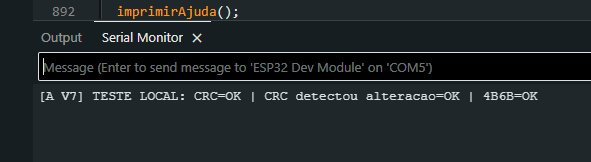
\includegraphics[width=\linewidth,height=150pt,keepaspectratio]{figuras/old_22_1.png}\caption{T01 — autoteste no circuito A.}\label{fig:old_22_1}\end{figure}
\begin{figure}[H]\centering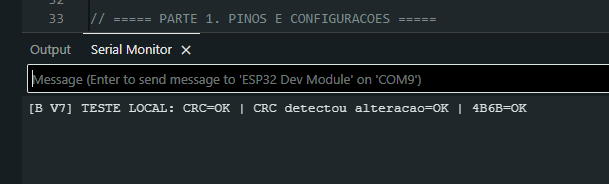
\includegraphics[width=\linewidth,height=135pt,keepaspectratio]{figuras/old_23_1.png}\caption{T01 — autoteste no circuito B.}\label{fig:old_23_1}\end{figure}
\begin{figure}[H]\centering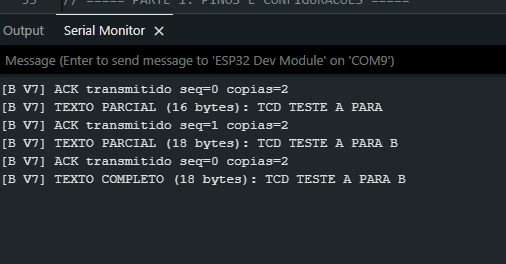
\includegraphics[width=\linewidth,height=180pt,keepaspectratio]{figuras/old_23_2.png}\caption{T02 — recepção da mensagem em B.}\label{fig:old_23_2}\end{figure}
\clearpage\subsection*{T03, T04 e T05}
\begin{figure}[H]\centering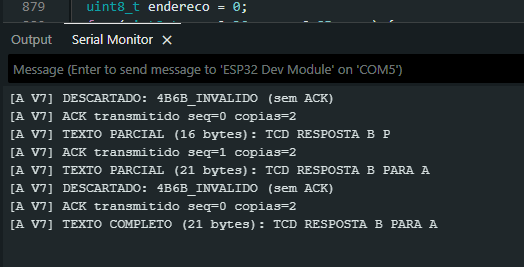
\includegraphics[width=\linewidth,height=190pt,keepaspectratio]{figuras/old_24_1.png}\caption{T03 — recepção da mensagem em A.}\label{fig:old_24_1}\end{figure}
\begin{figure}[H]\centering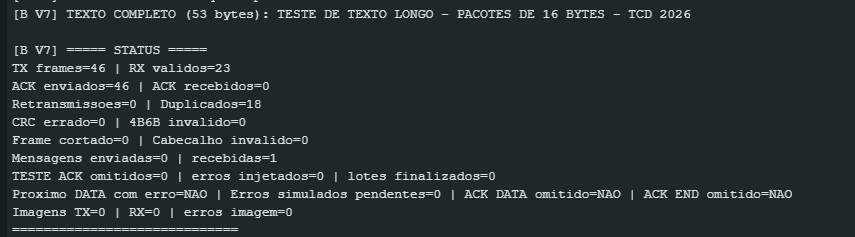
\includegraphics[width=\linewidth,height=145pt,keepaspectratio]{figuras/old_24_2.png}\caption{T04 — texto longo e contadores de B.}\label{fig:old_24_2}\end{figure}
\begin{figure}[H]\centering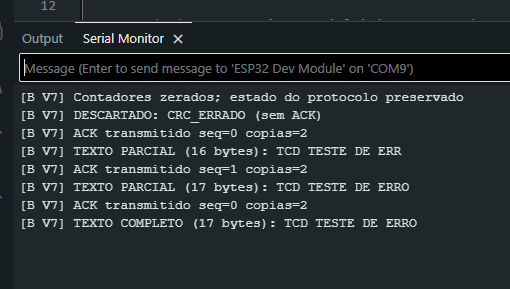
\includegraphics[width=\linewidth,height=195pt,keepaspectratio]{figuras/old_25_1.png}\caption{T05 — recepção do texto após erro simulado.}\label{fig:old_25_1}\end{figure}
\clearpage\subsection*{T06 e T07}
\begin{figure}[H]\centering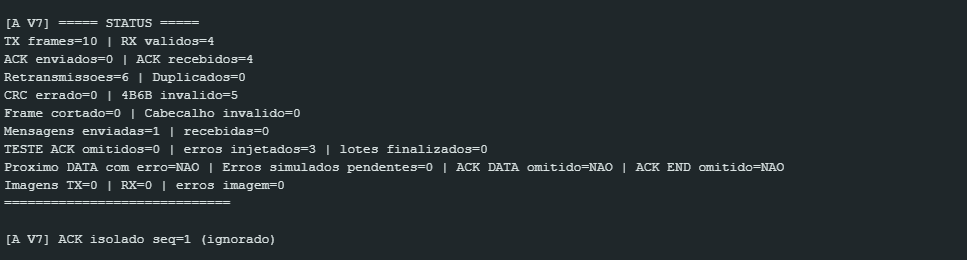
\includegraphics[width=\linewidth,height=130pt,keepaspectratio]{figuras/old_25_2.png}\caption{T06 — contadores do transmissor.}\label{fig:old_25_2}\end{figure}
\begin{figure}[H]\centering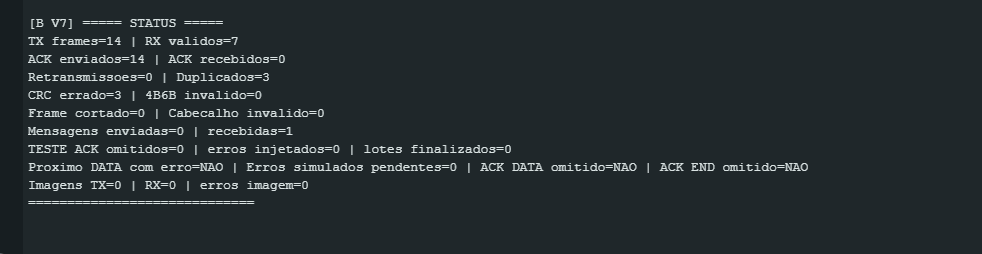
\includegraphics[width=\linewidth,height=130pt,keepaspectratio]{figuras/old_25_3.png}\caption{T06 — contadores do receptor, incluindo três erros CRC.}\label{fig:old_25_3}\end{figure}
\begin{figure}[H]\centering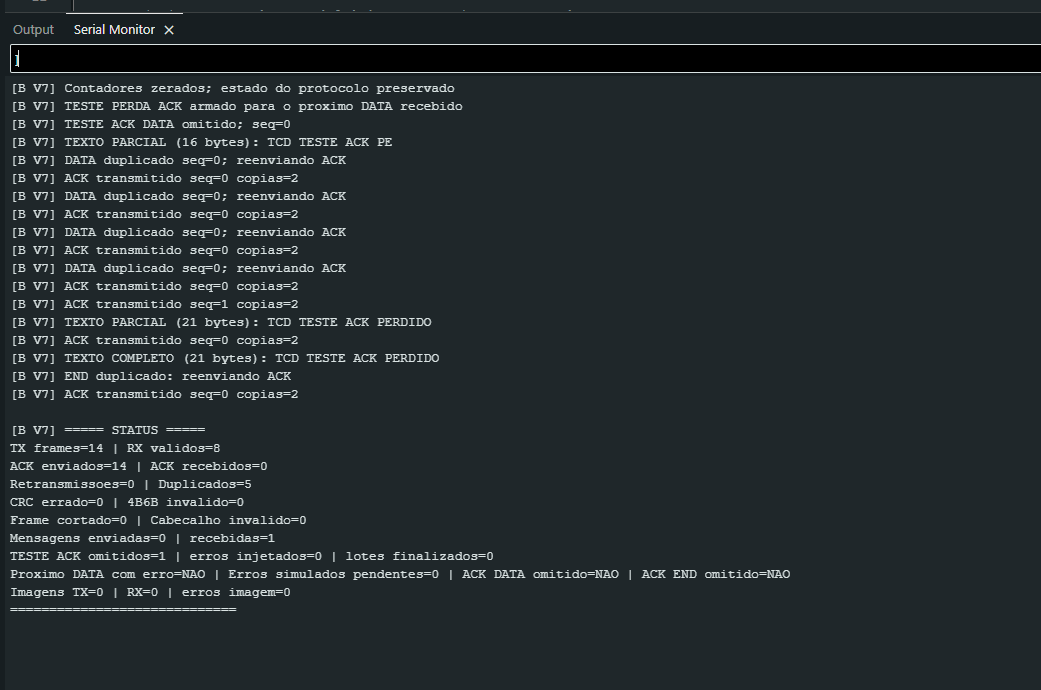
\includegraphics[width=\linewidth,height=230pt,keepaspectratio]{figuras/old_26_1.png}\caption{T07 — registro do transmissor.}\label{fig:old_26_1}\end{figure}
{\small T06: os três erros CRC estão registrados, mas o critério de duas mensagens não foi comprovado.\par}
\clearpage\subsection*{T07 e T08}
\begin{figure}[H]\centering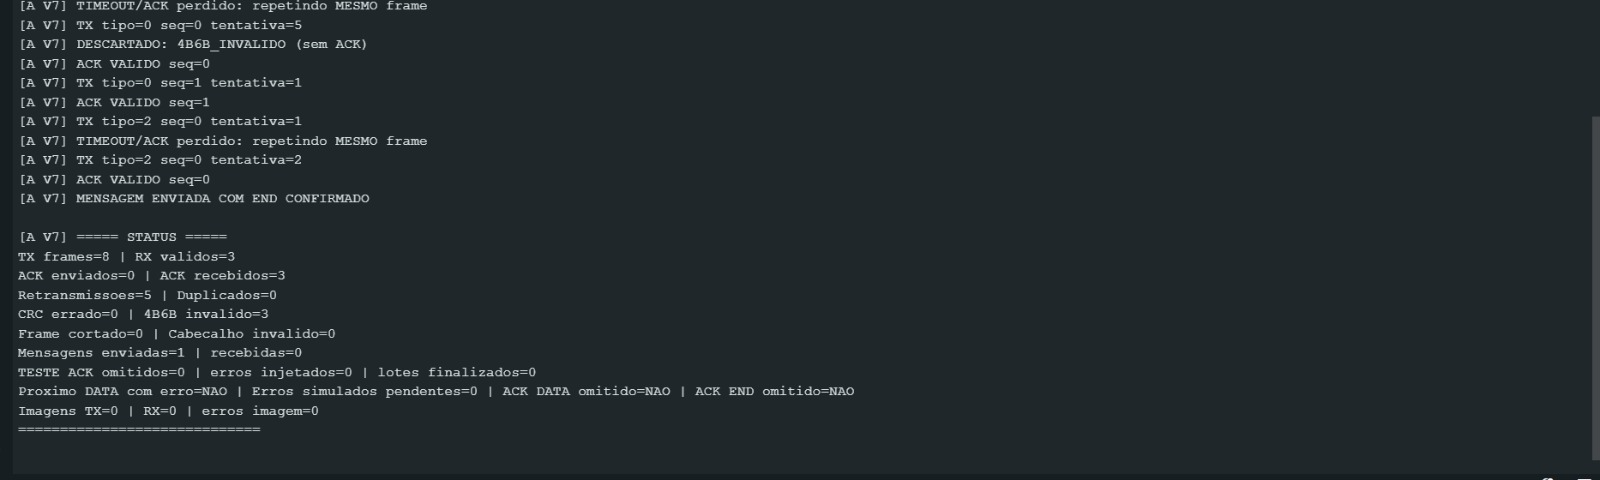
\includegraphics[width=\linewidth,height=185pt,keepaspectratio]{figuras/old_26_2.png}\caption{T07 — registro do receptor.}\label{fig:old_26_2}\end{figure}
\begin{figure}[H]\centering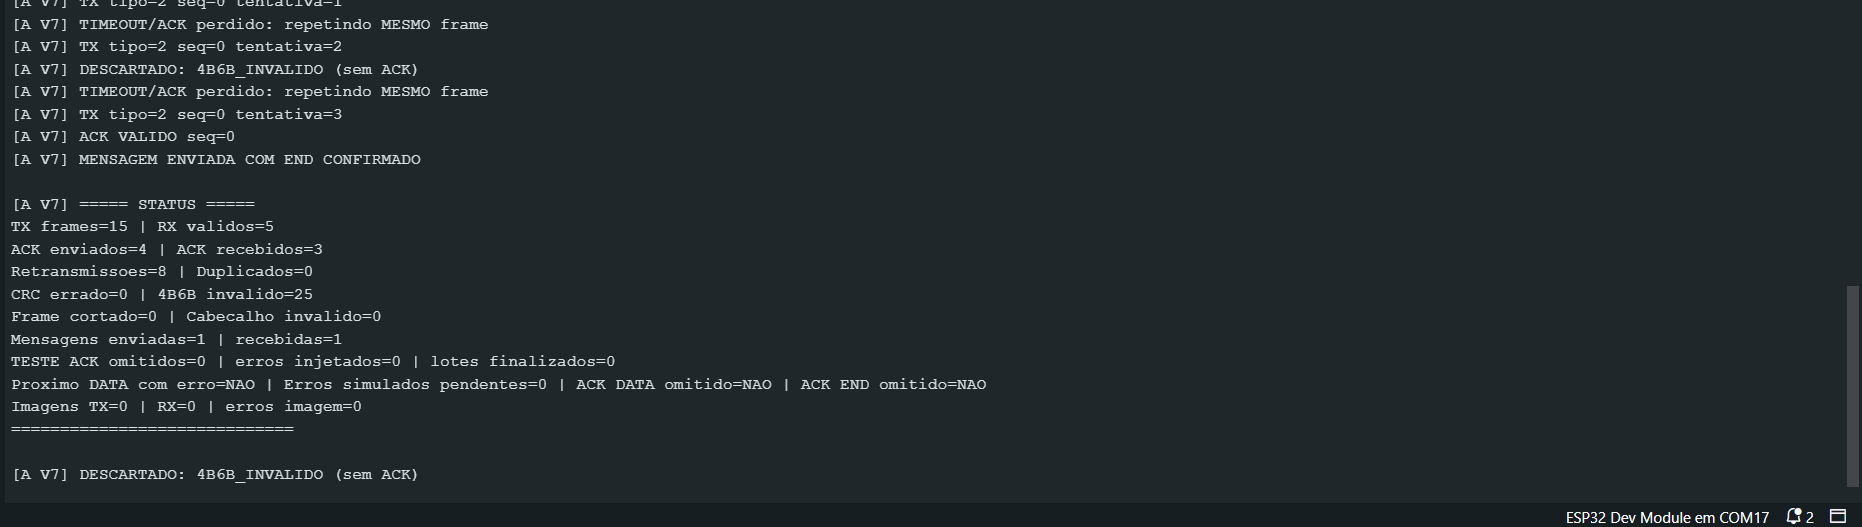
\includegraphics[width=\linewidth,height=185pt,keepaspectratio]{figuras/old_26_3.png}\caption{T08 — confirmação do END após retransmissão.}\label{fig:old_26_3}\end{figure}
\begin{figure}[H]\centering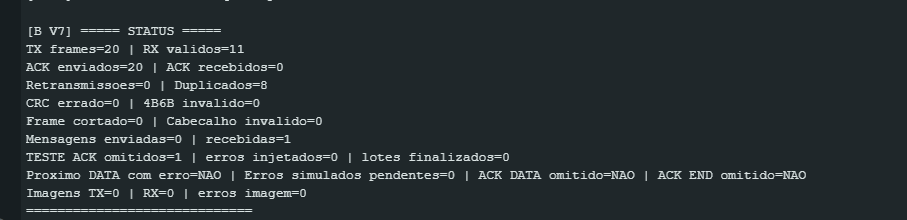
\includegraphics[width=\linewidth,height=180pt,keepaspectratio]{figuras/old_27_1.png}\caption{T08 — contadores do receptor e ACK omitido.}\label{fig:old_27_1}\end{figure}
\clearpage\subsection*{T09}
\begin{figure}[H]\centering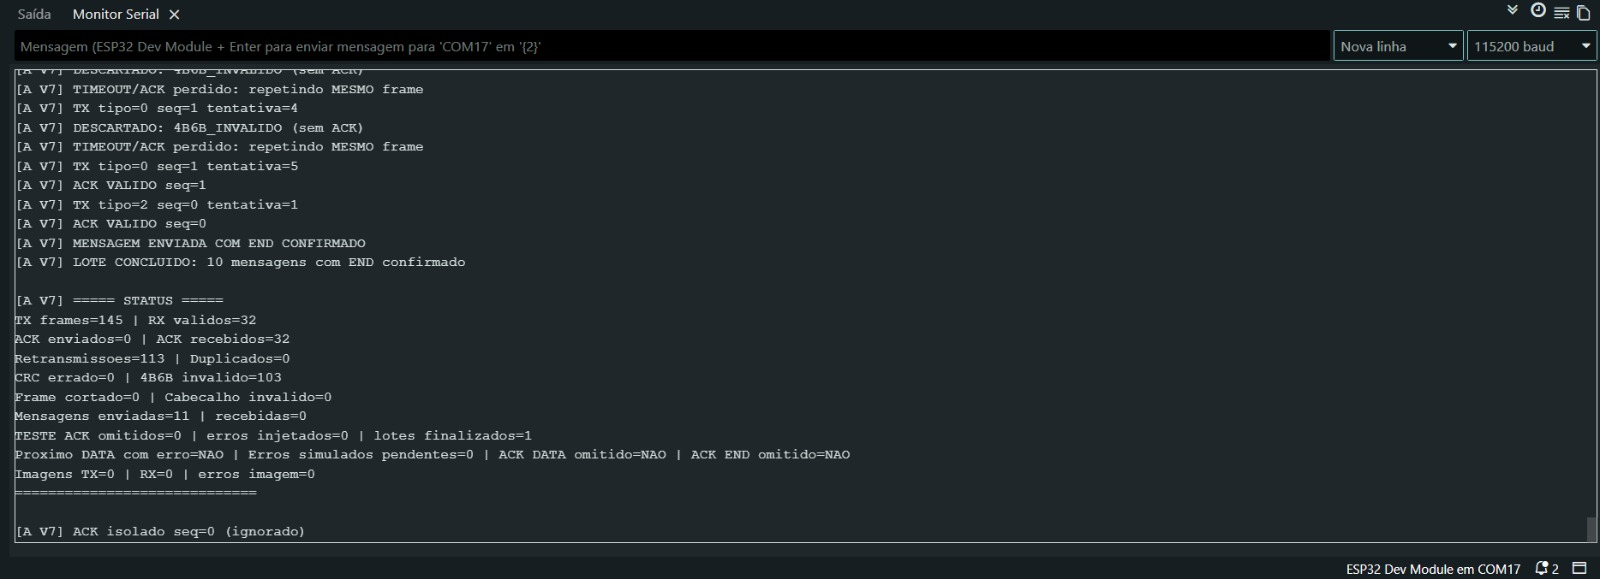
\includegraphics[width=\linewidth,height=180pt,keepaspectratio]{figuras/old_27_2.png}\caption{T09 — conclusão do lote no transmissor.}\label{fig:old_27_2}\end{figure}
\begin{figure}[H]\centering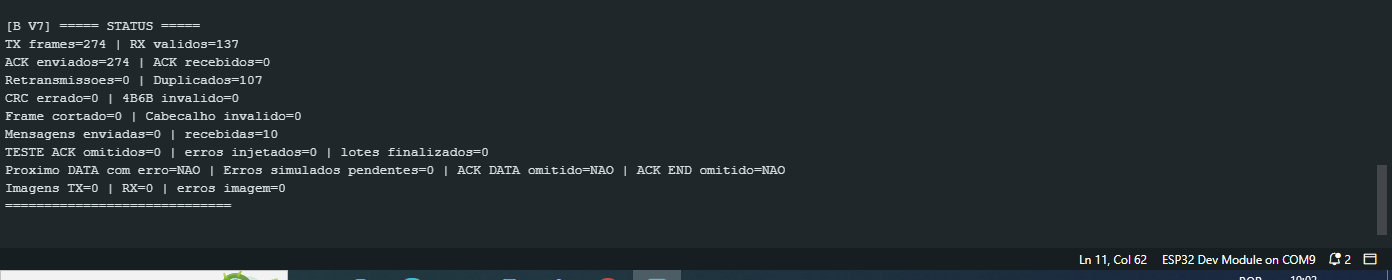
\includegraphics[width=\linewidth,height=180pt,keepaspectratio]{figuras/old_27_3.png}\caption{T09 — dez mensagens recebidas e duplicatas.}\label{fig:old_27_3}\end{figure}
\begin{figure}[H]\centering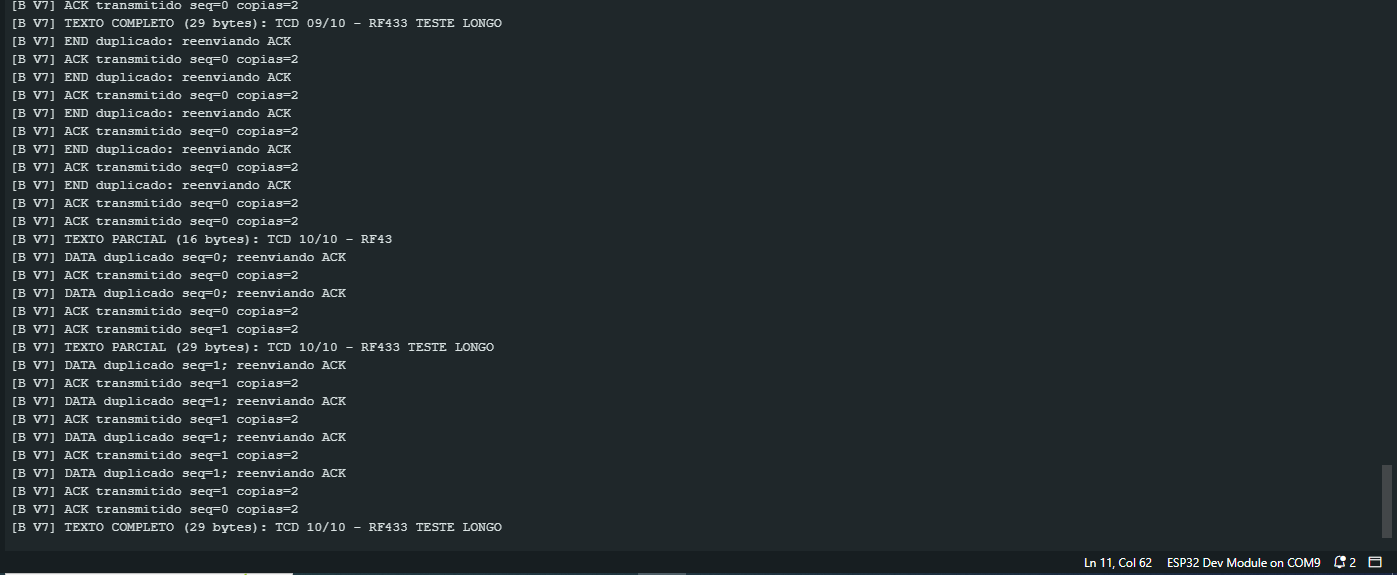
\includegraphics[width=\linewidth,height=180pt,keepaspectratio]{figuras/old_28_1.png}\caption{T09 — recepção das últimas mensagens do lote.}\label{fig:old_28_1}\end{figure}
{\small Os contadores do lote incluem atividade residual; os 113 reenvios não representam uma taxa isolada do T09.\par}
